\chapter{Практический раздел}

На рисунках~\ref{fig:screen}--\ref{fig:result} представлена работа программы для
нахождения предельных вероятностей нахождения системы в каждом
её состоянии по матрице интенсивностей переходов между ними.

\begin{figure}[ht]
    \centering
    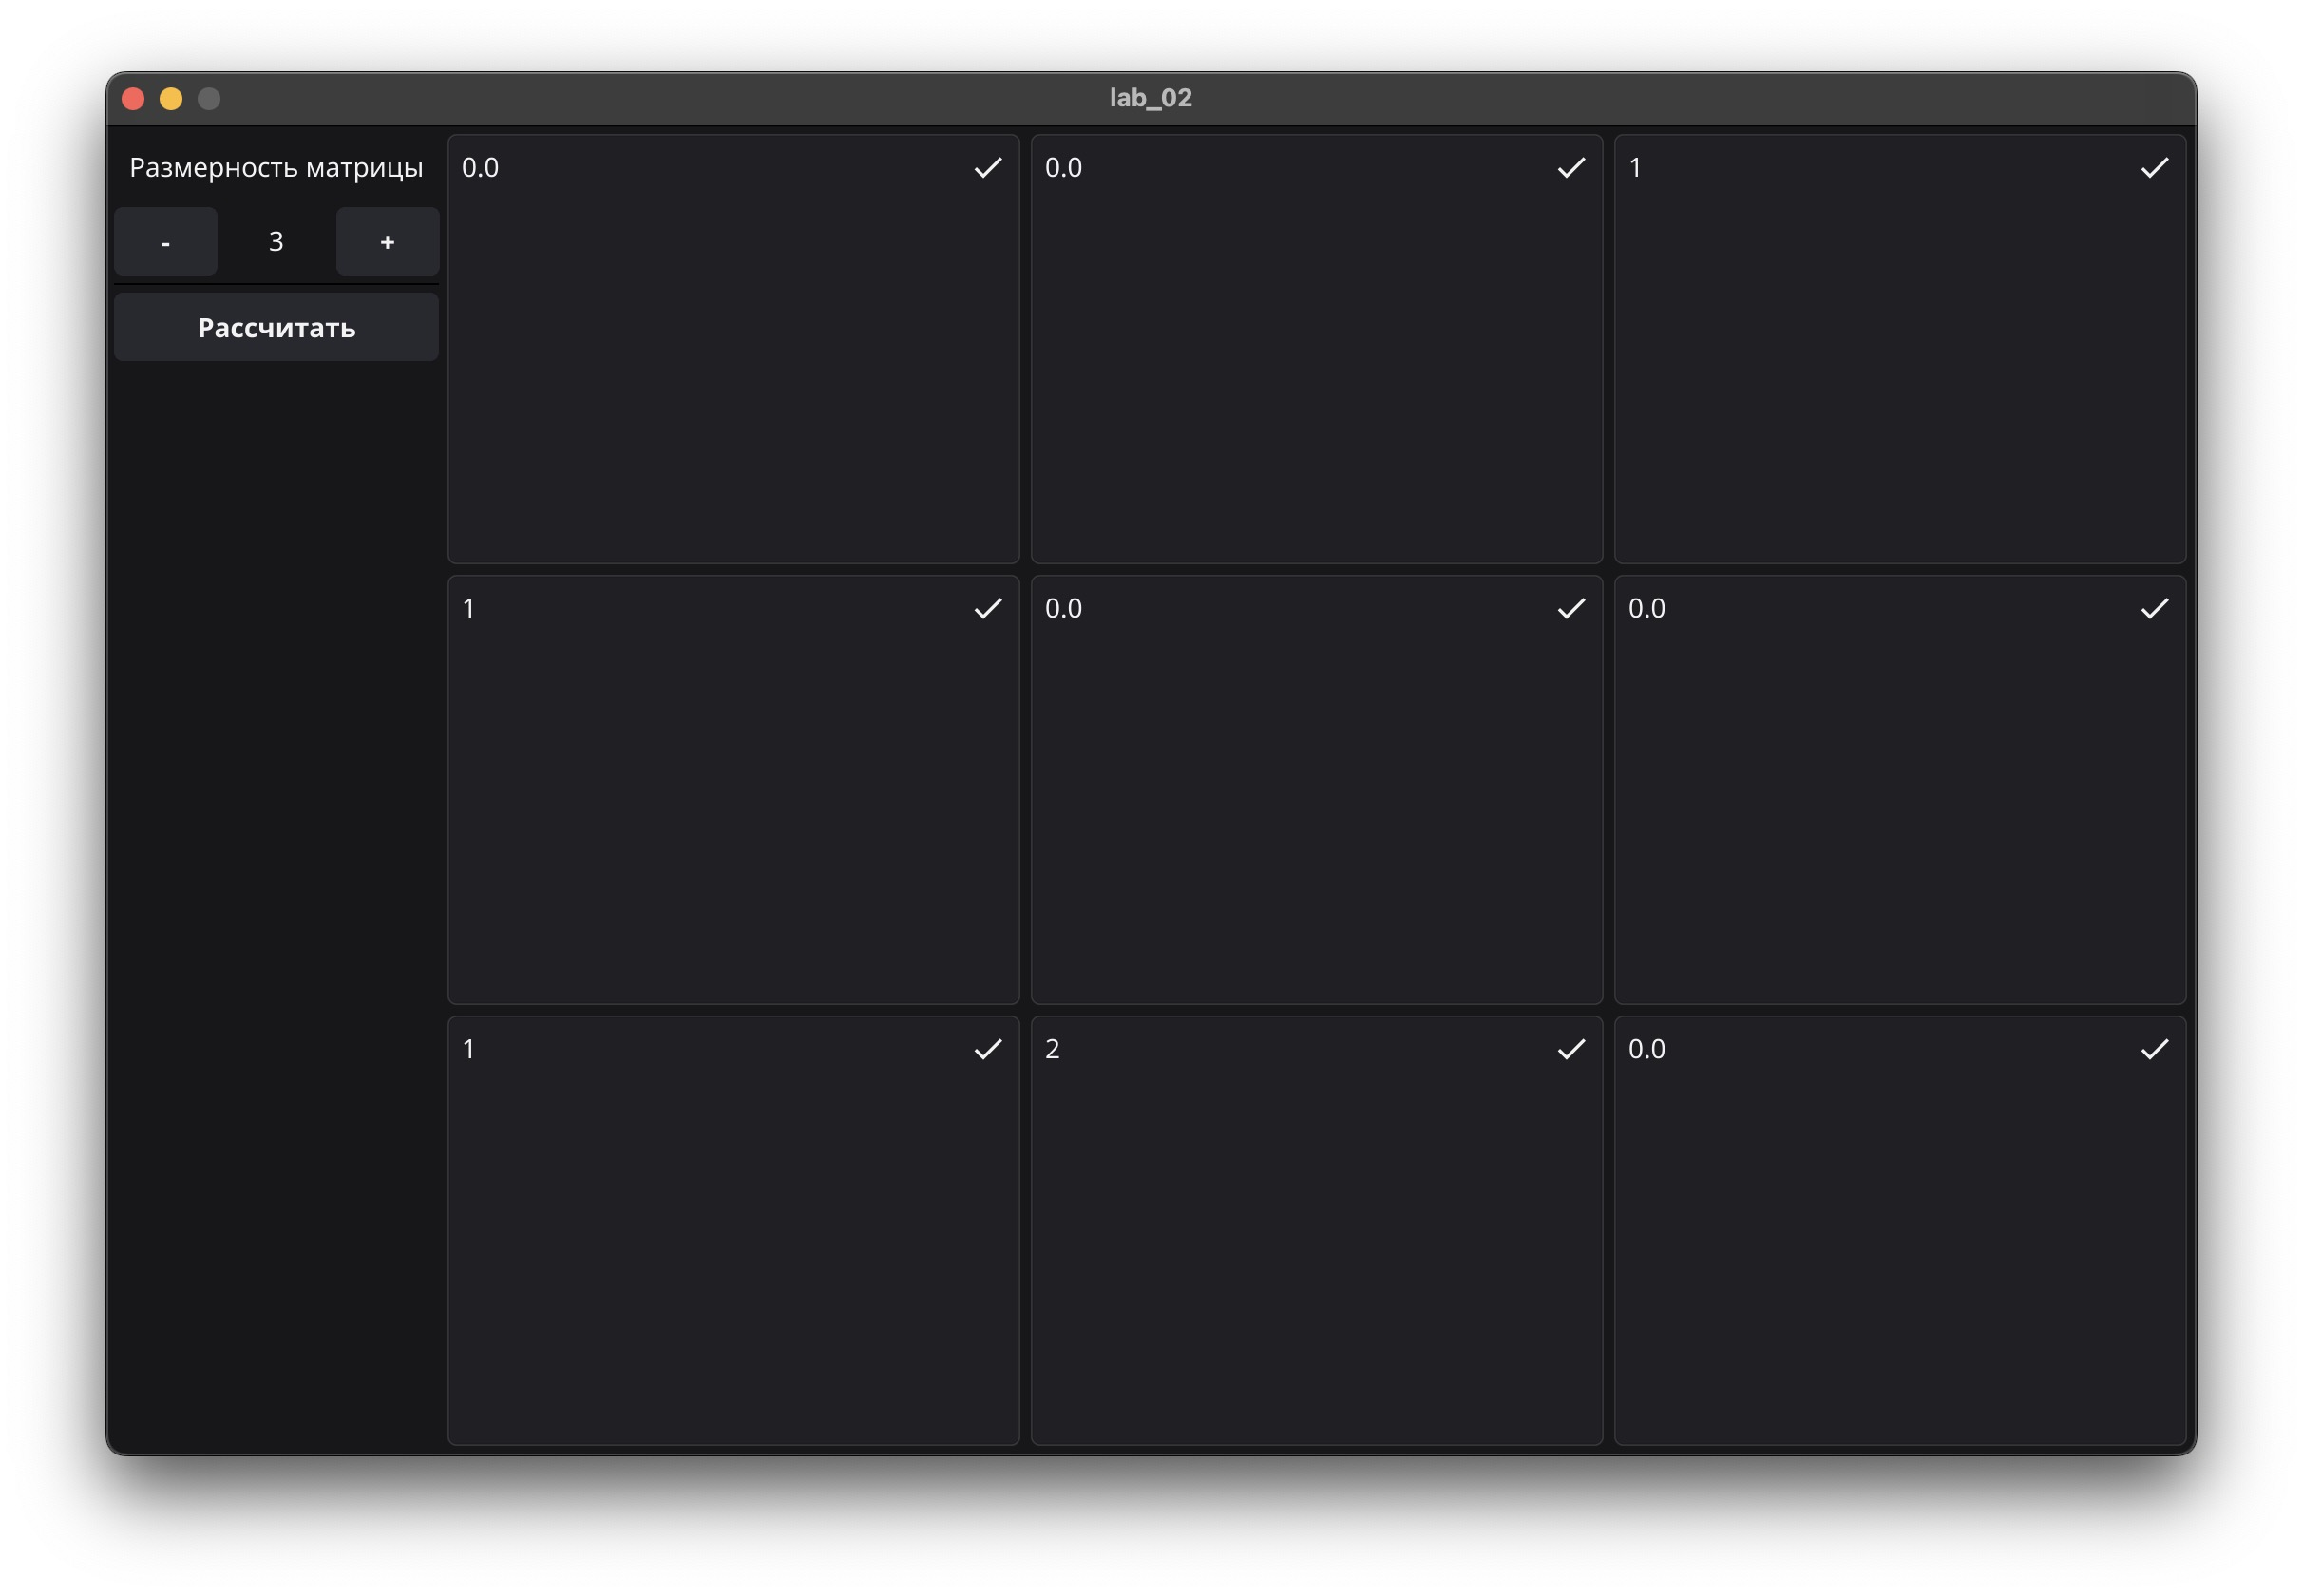
\includegraphics[width=0.95\textwidth]{assets/screen.jpeg}
    \caption{Демонстрация работы программы}
    \label{fig:screen}
\end{figure}

\begin{figure}[ht]
    \centering
    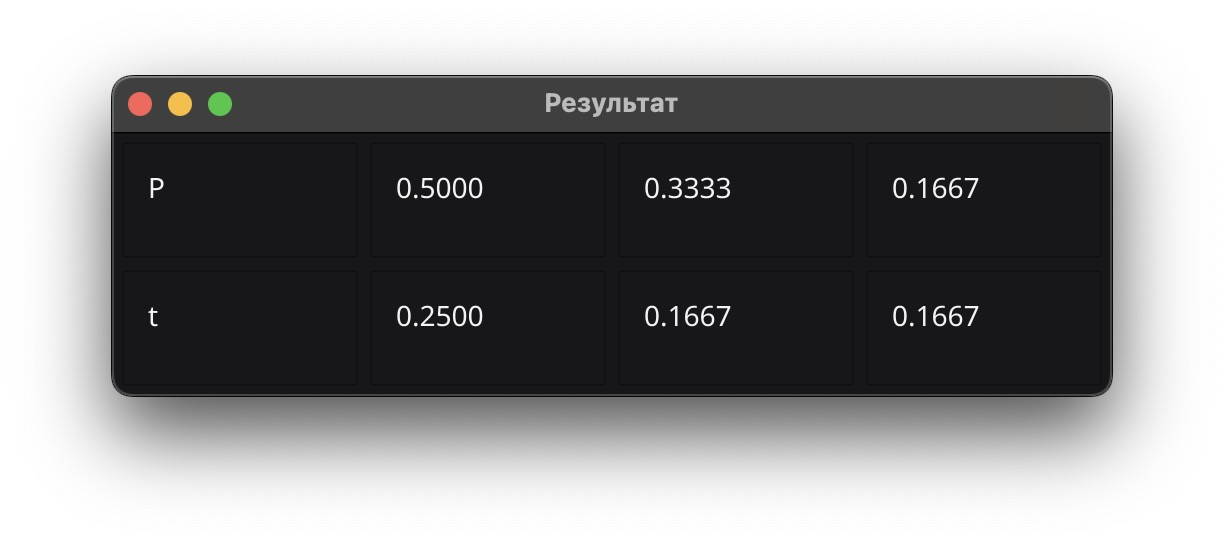
\includegraphics[width=0.95\textwidth]{assets/result.jpeg}
    \caption{Демонстрация результатов работы программы}
    \label{fig:result}
\end{figure}

\chapter{Вывод}

По результатам работы программы видно, что времена стабилизаций состояний значительно разнятся в зависимости от вероятностей состояний системы в начальный момент времени. Можно также заметить, что времена стабилизаций состояний уменьшаются с увеличением количества состояний и с увеличением значений интенсивностей переходов.
